\documentclass[10pt,aspectratio=169]{beamer}


\setbeamersize{text margin left=10pt, text margin right=10pt}
\usetheme{udea}

\setbeamercolor{block title}{bg=green!99,fg=white}


\usepackage{bm}
\usepackage{helvet}
\usepackage[english]{babel}
\usepackage[utf8]{inputenc}
\usepackage[T1]{fontenc}
%\usepackage{ragged2e}
\usepackage{etoolbox}
\usepackage{amssymb}
\usepackage{amsmath}
\usepackage{hyperref}
\usepackage{url}
\usepackage{graphics}
\usepackage{caption}
\usepackage{subfigure}
\captionsetup{compatibility=false}
\usepackage{ragged2e}
\usepackage{amsmath}
\usepackage{bibentry}
\usepackage{transparent}
%\usepackage{apalike}
\usefonttheme{professionalfonts}
\captionsetup[table]{name=Tabla}
\captionsetup[figure]{name=Figura}

\title[Titulo Corto]{\bf TÍTULO COMPLETO}
\institute[UdeA]{\bf Universidad de Antioquia, Medellín, Colombia}
\date[programa]{Doctorado en Ingeniería}
\author[N. Apellido]{{\bfseries PhD(c): } XXXX XXXXX\\ \vspace{1cm}  {\bfseries Director}: Ph.D. Tutor XXXXX}
\medskip
{\setbeamertemplate{footline}{}

\setbeamertemplate{footline}{
	\usebeamercolor[fg]{page number in head}%
	\usebeamerfont{page number in head}%
	\hspace{14cm}
	 \insertframenumber%/\inserttotalframenumber
	\vspace{14pt}
}


\definecolor{udea green}{rgb}{0.255,0.678,.286}
\setbeamercolor{frametitle}{fg=udea green}
\usepackage[maxcitenames=1, backend=bibtex, style=authoryear-comp]{biblatex}
\addbibresource{referencesFile.bib}
\newcommand{\customcite}[1]{{\color{udea green} (\citeauthor{#1}, \citeyear{#1})}}
\renewcommand*{\bibfont}{\scriptsize}

\DeclareMathOperator{\erf}{erf} \DeclareMathOperator{\real}{Re}
\DeclareMathOperator{\imag}{Im} \DeclareMathOperator{\tr}{tr}
\DeclareMathOperator{\cov}{cov} \DeclareMathOperator{\ex}{E}
\DeclareMathOperator{\var}{var}
\DeclareMathOperator{\bdiag}{blockdiag}
\DeclareMathOperator{\vecO}{vec} \DeclareMathOperator{\diag}{diag}
\DeclareMathOperator{\const}{const}
\DeclareMathOperator{\entropy}{H}
\providecommand{\abs}[1]{\lvert#1\rvert}
\newcommand{\dif}{\textrm{d}}

\newcommand{\boldgamma}{\bm{\gamma}}
\newcommand{\boldepsilon}{\bm{\epsilon}}
\newcommand{\boldlambda}{\bm{\lambda}}
\newcommand{\boldmu}{\bm{\mu}}
\newcommand{\boldSigma}{\bm{\Sigma}}
\newcommand{\boldg}{\mathbf{g}}
\newcommand{\boldphi}{\bm{\phi}}
\newcommand{\boldpi}{\bm{\pi}}
\newcommand{\boldZ}{\mathbf{Z}}
\newcommand{\boldY}{\mathbf{Y}}
\newcommand{\boldS}{\mathbf{S}}
\newcommand{\boldF}{\mathbf{F}}
\newcommand{\boldG}{\mathbf{G}}
\newcommand{\bolds}{\mathbf{s}}
\newcommand{\boldt}{\mathbf{t}}
\newcommand{\boldr}{\mathbf{r}}
\newcommand{\boldm}{\mathbf{m}}
\newcommand{\boldv}{\mathbf{v}}
\newcommand{\boldy}{\mathbf{y}} % output space
\newcommand{\boldx}{\mathbf{x}} % input space of the outputs
\newcommand{\boldz}{\mathbf{z}} % input space of the latent functions
\newcommand{\boldh}{\mathbf{h}} % lag
\newcommand{\boldk}{\mathbf{k}} % kernel or covariance
\newcommand{\boldK}{\mathbf{K}} % kernel or covariance
\newcommand{\boldf}{\mathbf{f}} % outputs without noise
\newcommand{\boldP}{\mathbf{P}} % coregionalization matrix
\newcommand{\boldL}{\mathbf{L}} % coregionalization matrix
\newcommand{\boldC}{\mathbf{C}} % coregionalization matrix
\newcommand{\boldM}{\mathbf{M}} % coregionalization matrix
\newcommand{\boldB}{\mathbf{B}} % coregionalization matrix
\newcommand{\boldA}{\mathbf{A}} % matrix of coeffcients a_{qi}^r
\newcommand{\boldu}{\mathbf{u}} % vector for latent function
\newcommand{\bolda}{\mathbf{a}} % vector for SLFM function
\newcommand{\boldAtilde}{\mathbf{\widetilde{A}}} % vector for SLFM function
\newcommand{\eye}{\mathbf{I}}   % identity matrix
\newcommand{\boldUpsi}{\bm{\Upsilon}}% vector of coefficients in th IMC
\newcommand{\boldupsi}{\bm{\upsilon}}% vector of coefficients in th IMC
\newcommand{\boldX}{\mathbf{X}} % The whole set of input vectors
\newcommand{\boldH}{\mathbf{H}} % The whole set of lag vectors
\newcommand{\boldI}{\mathbf{I}} % The identity matrix
\newcommand{\inputSpace}{\mathcal{X}} % The input space
\newcommand{\params}{\bm{\theta}} % Parameters of LMC model
\newcommand{\veC}{\textbf{\hspace{-0.001in}:}} % Simplified version of the vec operator (vec = :)
\newcommand{\preci}{\mathbf{P}}% Precision for the Gaussians
\newcommand{\dataset}{{\cal D}} % dataset
\newcommand{\gauss}{\mathcal{N}} % Gaussian density
\newcommand{\gammad}{\operatorname{Gamma}} % Gamma density
\newcommand{\betad}{\operatorname{Beta}} % Beta density
\newcommand{\bernd}{\operatorname{Bernoulli}} % Bernoulli density
\newcommand{\ones}{\mathbf{1}}
\newcommand{\zeros}{\mathbf{0}}

\usepackage{tikz}
\usetikzlibrary{shadings, snakes, calc,decorations.pathreplacing,positioning}
\usepackage{cancel}
\usepackage{braids}

\newcommand<>{\btikzset}[2]{\alt#3{\tikzset{#1}}{\tikzset{#2}}}

\tikzstyle{block}=[draw opacity=0.7,line width=1.4cm]
\tikzstyle{every picture}+=[remember picture]
\tikzstyle{na} = [baseline=-.5ex]

\usepackage{pgfplots}
%\pgfplotsset{compat=1.9}

% and optionally (as of Pgfplots 1.3):
\pgfplotsset{compat=newest}
\pgfplotsset{plot coordinates/math parser=false}
\newlength\figureheight
\newlength\figurewidth 
\newlength\globalheight
\newlength\fheight
\newlength\fwidth
\newlength\marksize

\makeatletter
\pgfplotsset{
	fenton/positive/.style={fill=white, draw=none},
	fenton/positive style/.style={/pgfplots/fenton/positive/.append style={#1}},
	fenton/negative/.style={fill=black, draw=none},
	fenton/negative style/.style={/pgfplots/fenton/negative/.append style={#1}},
	fenton/.style={
		axis background/.style={fill=white},
		only marks, no markers,
		scatter,
		axis equal image,
		xlabel = Dishes,
		ylabel = Clients,
		axis on top,
		major tick length=0pt,
		enlarge x limits={abs=0.5},
		enlarge y limits={abs=0.5},
		point meta=explicit,
		scatter/@pre marker code/.code={
			\pgfkeys{/pgf/fpu,/pgf/fpu/output format=fixed}
			\pgfmathsetmacro\normalisedsize{
				sqrt(
				abs(
				\pgfplotspointmeta / max(
				abs(\pgfplots@metamin),
				abs(\pgfplots@metamax)
				)
				)
				)
			}
			\pgfmathfloatifflags{\pgfplotspointmeta}{+}{
				\pgfplotsset{fenton/current value/.style=/pgfplots/fenton/positive}
			}{
				\pgfplotsset{fenton/current value/.style=/pgfplots/fenton/negative}
			}
			\path [/pgfplots/fenton/current value] ([scale=\normalisedsize]axis direction cs:-0.5,-0.5) rectangle ([scale=\normalisedsize]axis direction cs:0.5,0.5);   
		},
		scatter/@post marker code/.code={}
	}
}

\pgfdeclarelayer{background}
\pgfdeclarelayer{foreground}
\pgfsetlayers{background,main,foreground}
\tikzstyle{block} = [draw, rectangle, 
minimum height=1em, minimum width=1em]
\tikzstyle{blockg} = [draw, fill=green!20, rectangle, 
minimum height=10em, minimum width=2em, drop shadow]
\tikzstyle{blockr} = [draw, fill=red!20, rectangle, 
minimum height=10em, minimum width=2em, drop shadow]
\tikzstyle{blockb} = [draw, fill=blue!20, rectangle, 
minimum height=2em, minimum width=2em, drop shadow]
\tikzstyle{sum} = [draw, fill=blue!20, circle, node distance=1cm, drop shadow]
\tikzstyle{input} = [coordinate]
\tikzstyle{output} = [coordinate]
\tikzstyle{pinstyle} = [pin edge={to-,thin,black}]

\setbeamerfont{subsection in toc}{size=\footnotesize}
\setbeamerfont{section in toc}{size=\footnotesize}
\addtobeamertemplate{frametitle}{\vskip1.5ex}{}

\usepackage{ragged2e}
%\justifying

\begin{document}
%\begin{frame}
%	\centering
%	\bf\Large Modelos Probabilísticos Profundos para Detección de Espectro en Redes de Radio Cognitivas
%	\begin{figure}[htb]
%		\centering
%		\includegraphics[width=1\textwidth]{misc/pp2UQ}
%	\end{figure}
%\end{frame}

%\AtBeginSubsection[]
%{
%	\begin{frame}
%		\frametitle{Contenido}
%		\tableofcontents[currentsection,currentsubsection]
%	\end{frame}
%}

%\setbeamertemplate{frametitle}[default][left]


\AtBeginSection[] {
	\begin{frame}<beamer>
		\frametitle{\bf\Large Outline} %
		\tableofcontents[currentsection, 
		sectionstyle=show/shaded, 
		subsectionstyle=show/show/hide]  
	\end{frame}
}


%Fondo para la pagina del titulo
\setbeamertemplate{background}{
%	{\transparent{0.4}\includegraphics[width=0.8\textwidth]{misc/pp2UQ}}
	\tikz[overlay,remember picture]\node[at=(current page.center), opacity=0.2] {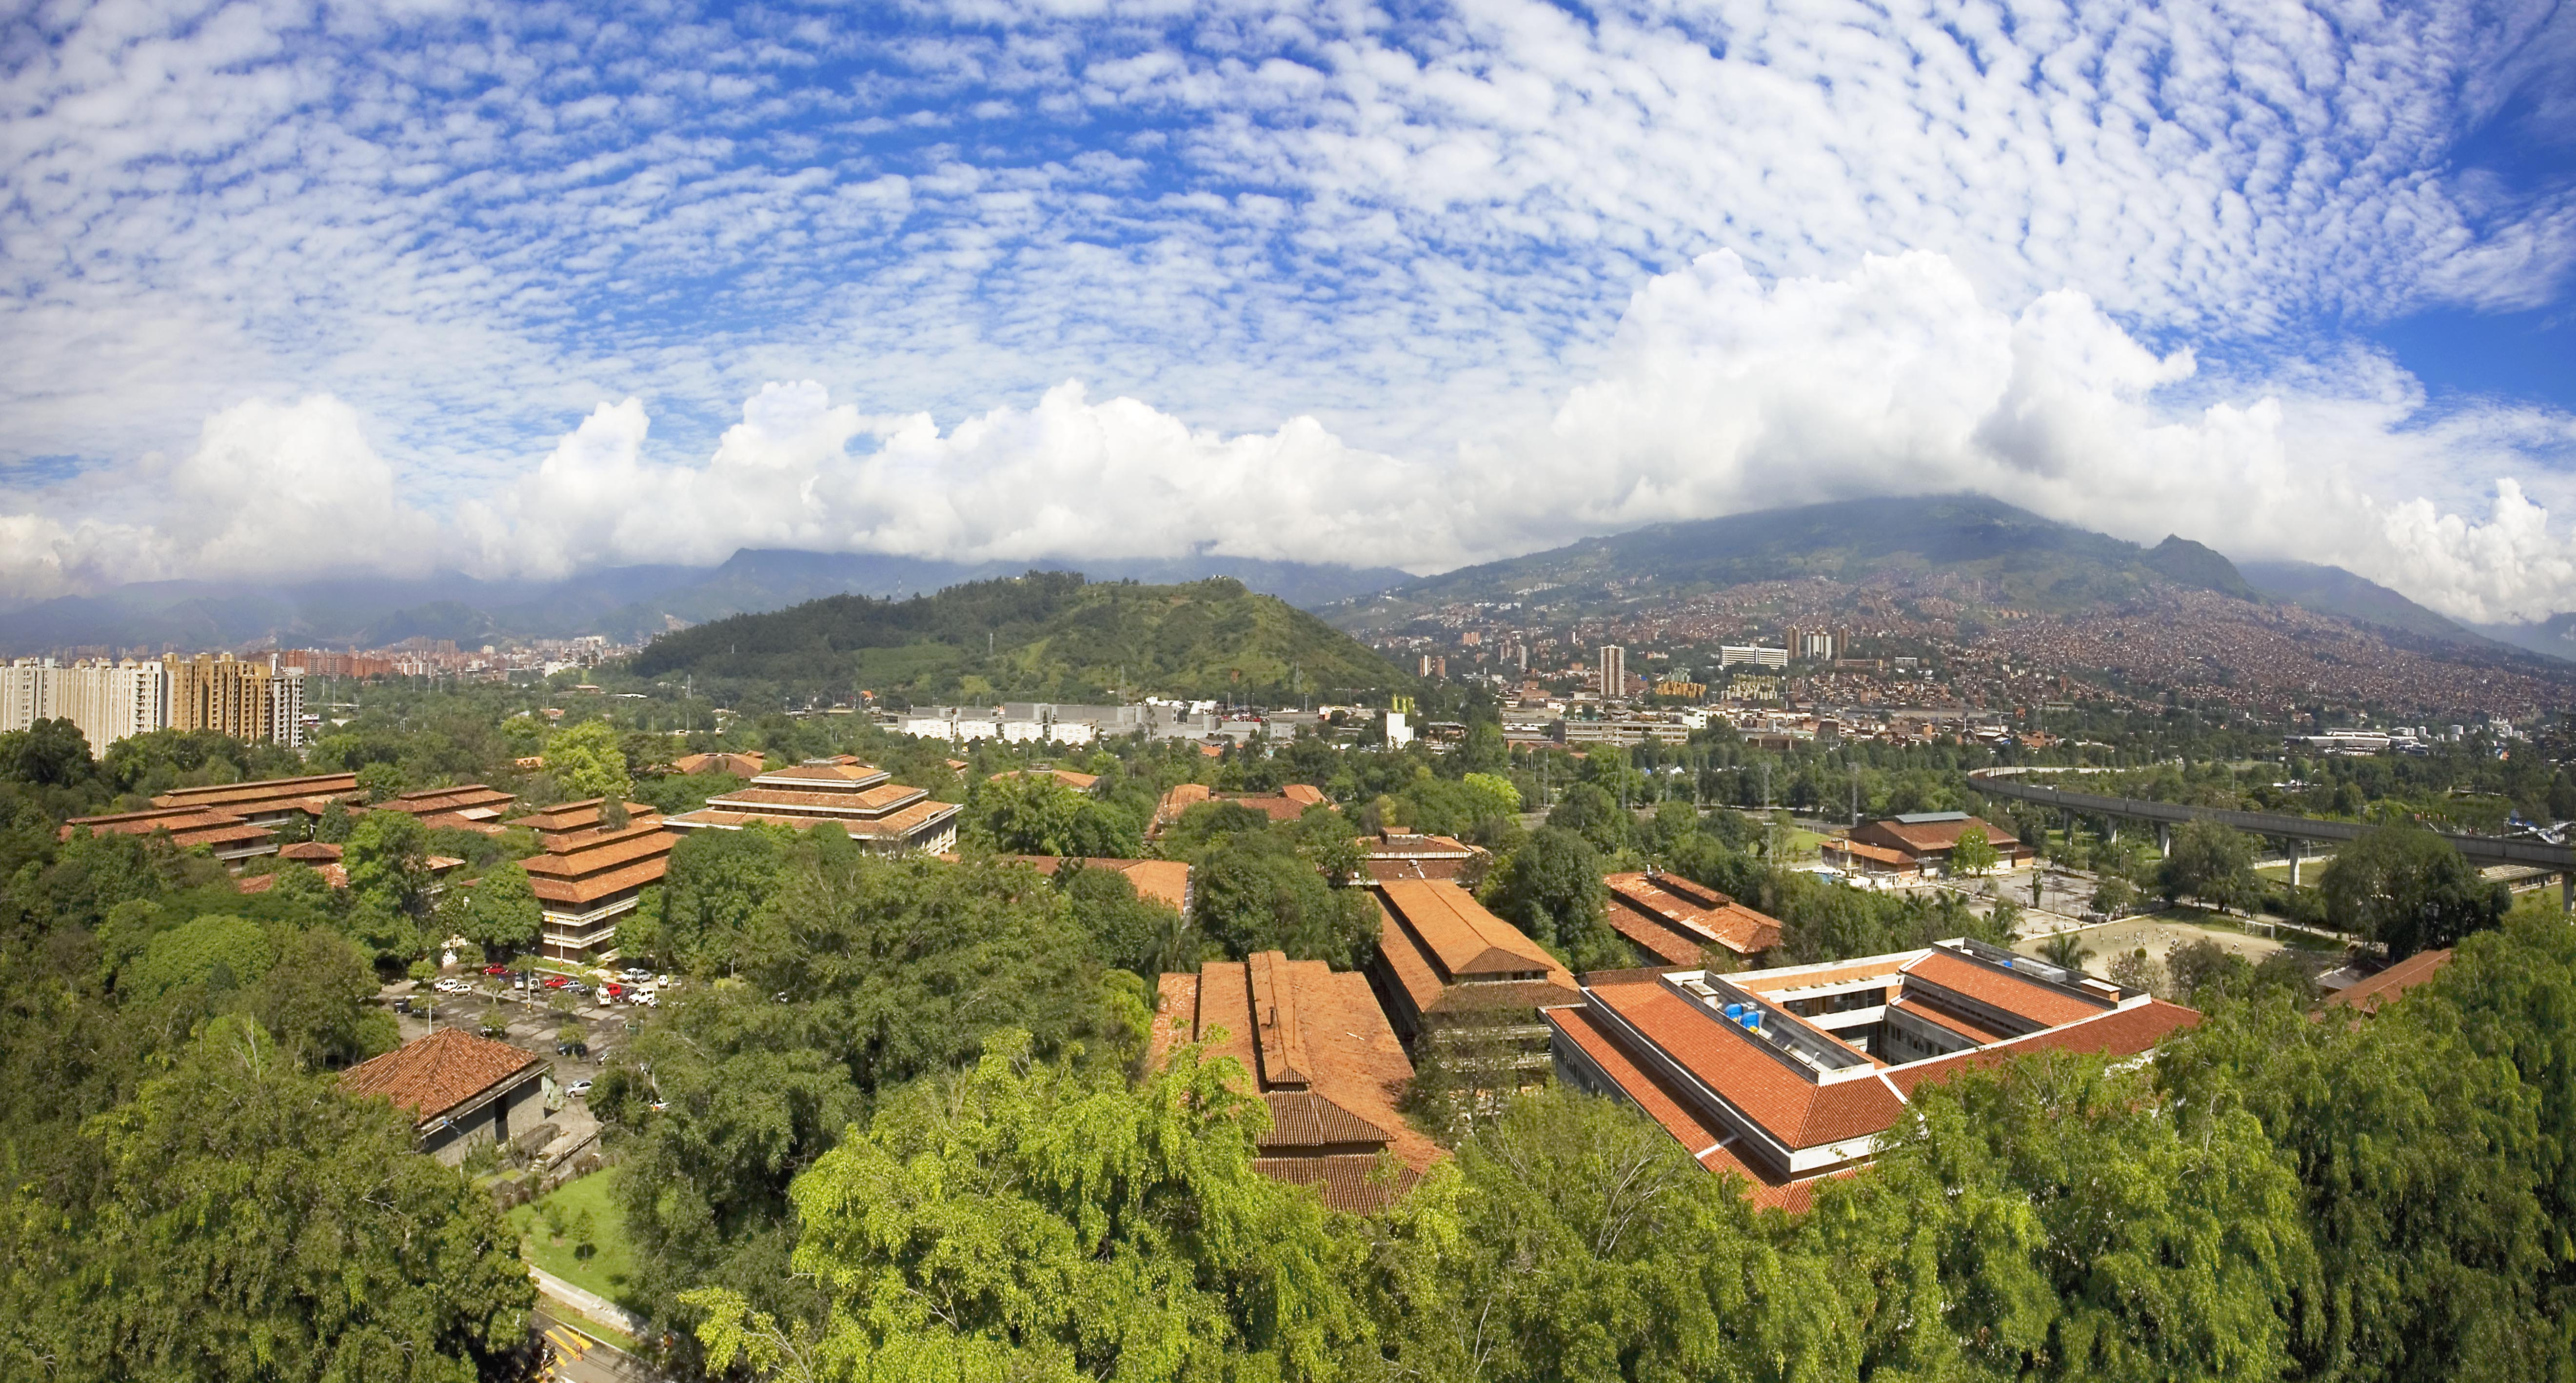
\includegraphics[height=\paperheight,width=\paperwidth]{bg/portadaUdeA}};
	\tikz[overlay,remember picture] 
	\node[at=(current page.south),anchor=south,inner sep=0pt] {
		
\includegraphics[width=1.05\linewidth]{bg/bottom_default_udea}};
	\tikz[overlay,remember picture] 
	\node[at=(current page.north),anchor=north,inner sep=0pt] {
		
\includegraphics[width=1.05\linewidth]{bg/top_title_udea}};
	
	}	
	
{\setbeamertemplate{footline}{}	%para eliminar el numero de la pagina
\begin{frame}[c]
	%{\transparent{0.4}\includegraphics[width=1\textwidth]{misc/pp2UQ}}
	\titlepage
\end{frame}
}

%Fondo para las demas paginas
\setbeamertemplate{background}{
	\tikz[overlay,remember picture] 
	\node[at=(current page.south),anchor=south,inner sep=0pt] {
		
\includegraphics[width=1.05\linewidth]{bg/bottom_title_udea}};
	
	\tikz[overlay,remember picture] 
	\node[at=(current page.north),anchor=north,inner sep=0pt] {
		
\includegraphics[width=1.05\linewidth]{bg/top_title_udea}};
	
}
%**************************************************************************
\section[]{Introducción}
\subsection[]{\tiny Motivación}
\begin{frame}[allowframebreaks]{\centering\bf\Large Motivación}
	
\end{frame}

\subsection[]{\tiny Planteamiento del problema}

\begin{frame}{\Large\bf Planteamiento del problema}
	
	\begin{block}{Bloque}
		XXXXXXXXx \customcite{bishop2006}
	\end{block}
\end{frame}

\begin{frame}{}
	\begin{block}{\bf\Large Pregunta de Investigación }
		\justifying
		\Large
		\textit{¿XXXXXXX?}
	\end{block}
	
\end{frame}

\subsection[]{\tiny Objetivos}
\begin{frame}{\bf\Large Objetivos}
	\begin{block}{\bf\Large General}
		%\begin{center}
		\justifying
		\Large
		XXXXXXXXXXXXXXXXXXXXXXXXxx
		%\end{center}
	\end{block}
	

	\begin{block}{\bf\Large Específicos}
		\begin{itemize}  
			%\justifying
			\large
			\item XXXXXXXXXXXXXXXxx
			%\pause
			\item XXXXXXXXXXXXXXX
			%\pause
			\item XXXXXXXXXXx
		\end{itemize}
	\end{block}
\end{frame}

%%%%%%%%%%%%%%%%%%%%%%%%%%

\begin{frame}[allowframebreaks]{\bf\Large Referencias}
	\begin{columns}
		\begin{column}{0.9\linewidth}
		\printbibliography
		%\bibliographystyle{plain}
		%\bibliography{references}
		\end{column}
	\end{columns}
%	\tiny

\end{frame}

\begin{frame}
	\centering
	\vspace{0.5cm}
	\bf\huge ¿Preguntas?
	
	\begin{tikzpicture}
		\node [opacity=0.4] (0,0) {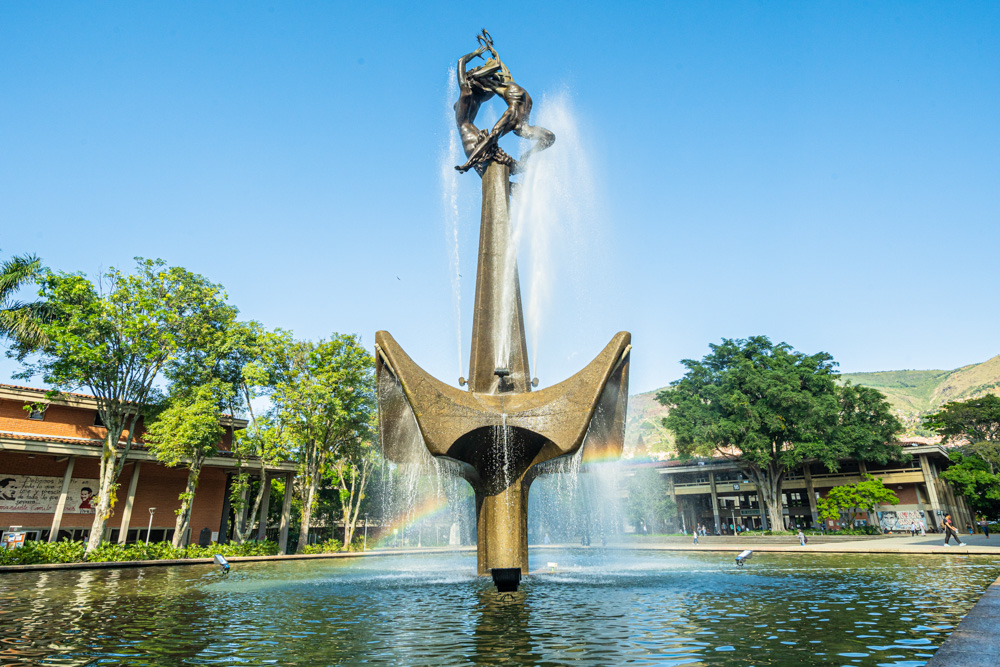
\includegraphics[width=0.5\linewidth]{bg/UdeABg}};
		%\node [opacity=0.2] (0,0) {\scalebox{5.0}{\textcolor{green}{MensajeOpcional}}};
	\end{tikzpicture}
%	\begin{figure}[htb]
%		\centering
%		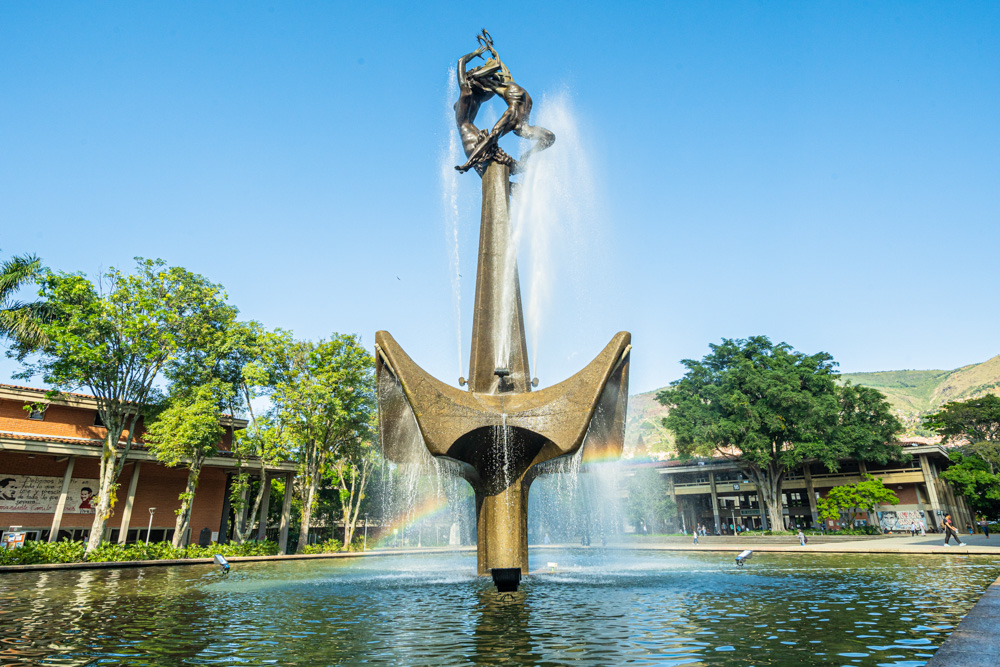
\includegraphics[width=0.7\textwidth]{bg/UdeABg}
%	\end{figure}
\end{frame}

\begin{frame}
	\centering
	%\vspace{0.5cm}
	%\bf\huge Gracias!
	\begin{figure}
		\centering
		
\includegraphics[width=1\textwidth]{bg/despedida_udea}
	\end{figure}
\end{frame}

\end{document}

